\documentclass[tikz]{standalone}

\begin{document}
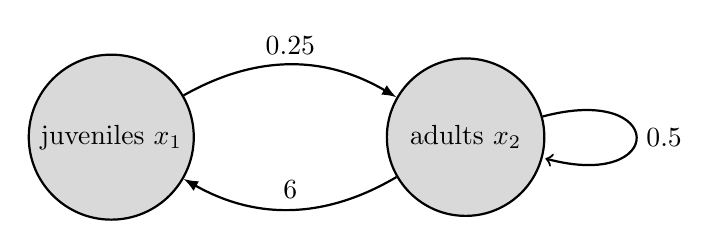
\begin{tikzpicture}[thick, class/.style={circle,draw,minimum size=2cm,fill=gray!30,align=center},scale=3]
  \node[class] (A) at ( 0.75,0.75) {adults \(x_2\)};
  \node[class] (J) at (-0.75,0.75) {juveniles \(x_1\)};
                %
  \path[-latex] (J) edge [bend left] node[above] {\(0.25\)} (A);
  \path[-latex] (A) edge [bend left] node[above] {\(6\)} (J);
  \path[-latex] (A) edge [loop right] node[right] {\(0.5\)} (A);  
\end{tikzpicture}
\end{document}
